\documentclass[]{article}
\usepackage{fullpage}
\usepackage[authoryear]{natbib}
\usepackage{setspace}
    \doublespacing
\usepackage{hyperref}
\hypersetup{
    colorlinks,
    citecolor=black,
    filecolor=black,
    linkcolor=cyan,
    urlcolor=cyan
}
\usepackage{amssymb,amsmath}
\usepackage{bm}
\usepackage{dcolumn}
\usepackage{booktabs}
\usepackage{url}
\usepackage{tikz}
\usepackage{todonotes}
\usepackage[utf8]{inputenc}
\usepackage{graphicx}
\usepackage{longtable}
\usepackage{todonotes}
\usepackage{lscape}
\usepackage{float}

\usepackage[margins]{trackchanges}


\title{Fiscal Rule Stretching in the European Union}

\author{Christopher Gandrud \\ \emph{City University London} \\ \emph{Hertie School of Governance}\footnote{Christopher Gandrud is Lecturer in Quantitative International Political Economy at City University London and Post-doctoral fellow at the Hertie School of Governance. Please contact him at Rhind Building, City University London, EC1V 0HB, London, United Kingdom
(\href{mailto:christopher.gandrud@city.ac.uk}{\nolinkurl{christopher.gandrud@city.ac.uk}}). Mark Hallerberg is Professor of Public Management and Political Economy at the Hertie School of Governance, Friedrichstrasse 180, Berlin 10117, Germany (\href{mailto:hallerberg@hertie-school.org}{\nolinkurl{hallerberg@hertie-school.org}}). Thank you to workshop participants at Texas A \& M University. This work was supported by the Deutsche Forschungsgemeinschaft under grant number HA5996/2-1. Replication material can be found at: \url{https://github.com/christophergandrud/Eurostat_revisions}.}
\and
Mark Hallerberg \\ \emph{Hertie School of Governance}}

\begin{document}

\maketitle

\addeditor{MH}
\addeditor{CG}

\begin{center}
    \textbf{Working draft. Comments and suggestions very welcome.}
\end{center}

\begin{abstract}
Elected governments have incentives to stretch accounting rules. Doing so improves the government’s appearance to cost-conscious voters and fiscally important international institutions, especially in the European Union where there are externally imposed budget limits. We expect rule stretching to be especially prevalent during periods of financial market stress and crisis given these events' large costs and that policy responses are often not obviously classifiable as being inside or outside of the government sector. To test these propositions, we examine debt data revisions made by the European statistical agency--Eurostat. We find that debt figures are more likely to be revised upwards for countries facing European Union budget enforcement and years close to national elections, especially when unscheduled. These election effects are heightened by financial market stress. Our research underlines the importance of having a vigilant and politically independent government statistical agency to ensure reliable government finance statistics.
\end{abstract}


\textbf{Keywords:} fiscal policy, European Union, financial crisis, electoral budget cycles, Eurostat


\section{Introduction}

We examine why governments stretch the rules when they determine how policies impact their debts, especially during periods of financial market stress and turmoil. By `rule stretching' we mean that when the fiscal implications of a policy are potentially ambiguous, a decision is made to minimise its affects on the public balance sheet. This research question impacts a number of political science literatures in interesting ways. One strand examines the relationship between the reporting of data and the quality of governance \cite[e.g.][]{Hollyer2014}. \cite{Alt2014} explore the relationship among the transparency of fiscal data, elections, and pressure from the European Union. They argue that European Union member states were more likely to violate the Eurostat statistical agency's rules for reporting budget data when fiscal transparency was low and when it was an election year in ways that made the government look better to voters. A related strand focuses on the economic vote and whether or not voters notice or incorporate information about these revisions into their decisions. \cite{KayserLeininger2015} find that the press, and voters as a result, do not pay attention to revised figures.

Our paper builds on insights on data revisions by Kayser and Leininger and on elections and fiscal transparency by Alt, Lassen, and Wehner to explore the implications of their arguments for government action.  If voters care most about reported, rather than actual, figures then governments have an incentive to manipulate them before elections. One would expect greater manipulations in ways that make the government's stewardship of the public balance sheet look better as elections approach. There is also an indirect electoral channel that runs through international institutions and investors in European Union member states. \cite{vonHagenWolff2006} argue that member states are more likely to use creative accounting when their deficits approach three percent of GDP. The reason is that such countries face a supranational fiscal rule under the Stability and Growth Pact where they are expected to run budget deficits less than three percent of GDP. Fiscal rule stretching could give governments more room to not have to cut back in areas voters care about in order to meet internationally agreed commitments. Governments may similarly rule stretch in order to maintain an attractive balance sheet for foreign sovereign bond investors, thus allowing them to fund programs that voters want. In more recent work that comes closest to our approach, \cite{DeCastro2013} find that most European Union member states are more likely to understate their deficits, that this behavior is more common in pre-electoral periods, and less common with more stringent fiscal rules in place. We expand this research in several important ways.

First, we consider the effects of financial crises on the likelihood of governments to rule stretch. During a financial crisis, electorally motivated fiscal rule-stretching is potentially even more pronounced. Financial crises substantially strain public budgets as economic activity and so tax revenue decrease, while bank bailout policies incur significant expenses. At the same time, many tools commonly used to respond to financial crises--guarantees, liquidity assistance, public asset management companies--have potentially ambiguous fiscal implications. During a financial crisis politicians have even stronger incentives and capabilities to rule stretch around elections.

Second, unlike \cite{DeCastro2013}, who discuss any revisions to deficit figures, we focus on  revisions to debt figures, and in particular on those that Eurostat requires.
%\add[CG]{ When liabilities are realized these costs can be shifted by politicians such that it does not effect the deficit, but does impact the debt. For example, in December 2015 the Portuguese government was able to provide 1.8 billion euros in support to the troubled bank Banif by having another bank--Santander Totta--purchase 1.8 billion euros of government 10-year notes. The country's debt increased as a result of this maneuver, but not its deficit.} \todo{Need to cite Eurointelligence}
There are several advantages of focusing debt data revisions made by Eurostat. First, as \cite{vonHagenWolff2006} note for so-called `stock-flow' adjustments and \cite{MilesiMoriyama2006}  separately note using a balance sheet approach, there are many operations that governments can use that change deficit figures without any need for revisions of deficit figures. This suggests that \cite{DeCastro2013} may underplay the extent of the manipulation. Note that the operations the authors above describe reduce the reported deficit, but do not affect the gross debt burden. It is in this part of government accounts where we expect to find evidence of rule stretching. Additionally, we focus on debt figures because this is were we anticipate the most fiscal rule stretching during financial crises. Policies such as bank guarantees, liquidity assistance, and nationalizations have potentially ambiguous effects on the public debt, largely because they create contingent rather than immediately realized liabilities which can be difficult to catergorize. We rely on Eurostat-mandated changes; \cite{DeCastro2013} find that Eurostat catches the bias downward in deficit figures; once Eurostat revisions are excluded, the remaining revisions are essentially noise. Eurostat is also meant to enforce a common set of rules, which provides a common metric to compare revisions across member states. The final main contrast with previous research concerns the countries and years included in our sample--we use a data set of the EU-28 members and include data from the the period 2003-2013, which allows us to consider the effects of the financial crisis.\footnote{\cite{DeCastro2013} only looked at the EU-15 and their sample ended in 2008. The one downside of including our measure of financial stress, which we explain in more detail below, is that we do not have data for this variable before 2003.}

%We explore two main alternative hypotheses. The first alternative focuses on `shocks' to the economy, which in turn affect government statistics. Countries with more shocks may engage in more revisions, with the bias depending upon the nature of the shocks (positive or negative). One can expect that the shocks are symmetrical, where the greater the shock the more the potential revision, or that one direction requires more revisions, with  the relative elasticities of taxes making one direction more volatile than another. This would be the standard `economic' argument. These revisions, however, should be due to `economic' effects and not conscious government manipulation. The forecasting literature in economics includes such measures. The second one considers institutional arguments about who generates the numbers. In some countries, the government does the reporting, while in others an independent body plays this role. Of course, these three arguments may be related in theoretically interesting ways. For example, a country experiencing a positive shock may be more likely to call an election in countries where elections are unscheduled.

Our dataset is composed only of European Union member states. This is useful for several reasons. They all technically fall under the same set of fiscal rules--the European System of Accounts (ESA)--, although the penalties are theoretically greater for euro member states.  Importantly for our analysis, national agencies produce the initial fiscal figures. They report this data to one body--Eurostat--which then evaluates the data and enforces the accounting standards by revising governments' original data. This means that differences across countries in initial reporting are not due to different accounting rules, but instead  different interpretations of these rules. Institutionally, these countries are all parliamentary or semi-presidential systems where elections are crucial for the formation of governments.

%We find that member state debt figures are more likely to be revised upwards for years close to national elections, especially when these are unscheduled. This suggests that governments are more prone to rule stretch closer to elections. They tend to `low ball' how much policies will cost closer to elections, which leads to an upward Eurostat revision in later years. Our research underlines the importance of having a vigilant and politically independent government statistical agency during periods of financial market stress to ensure reliable government finance statistics.

\section{Political budget cycles and fiscal rule stretching}

The revision of government-reported statistics is of interest for several reasons.

The reporting of statistics, or the lack of it, may tell one about the quality of the overall governance of a given country. \cite{Hollyer2014} argue that the lack of reporting is not random. They record the availability of data for 125 countries over a thirty-year period. They analyse this data with a Bayesian Item Response model to create a transparency index. They then use this index to predict the quality of governance in autocracies. In other work, they anticipate that this type of transparency affects government accountability as well as collective action \citep{hollyerforthcoming}.\footnote{\cite{jervin2013} tells a similar story for African countries. The quality of data is generally good when governments have state capacity to provide them. When those governments get into trouble, however, so that their capacity declines the quality of the data also drops.}

While \cite{Hollyer2014} consider how voters might react under conditions when they get data and when they do not, there is a separate literature on the economic vote that assumes that voters have no trouble accessing regular data on the state of the economy and they use this to decide about the competence of the government in managing economic policy. One debate considers whether voters are prospective or retrospective. On the latter, the assumption is that voters observe outcomes, and they decide whether to support the incumbent government. In response to the strong assumptions about voter knowledge, there is a growing literature on `real-time fiscal policy'. \cite{KayserLeininger2015} argue that the press ignores revisions to data. Moreover, \cite{kayser_peress} find that voters pay particular attention to data they do not experience themselves. They observe unemployment, for example, but they do not observe economic growth and rely on reported figures when making decisions about which party to support. In our case, we are interested in government fiscal data that only the government can report. If one combines the insights in the two papers, they suggest that voters make decisions on the first set of data they see. This would make manipulation of such data potentially rewarding for governments that seek to remain in office.

\subsection{Fiscal stretching for a domestic audience}

We build on this insight for our core argument. Following \cite{nordhaus1975} as well as \cite{Alt2014}, one would anticipate that there are opportunistic business cycles where governments manipulate macro-economic tools at their disposal in an effort to make the economy look better before an election. \cite{clark2003} finds the tools a government uses depends upon the logic of the Mundell-Fleming model: if one assumes that capital is mobile, a government relies on monetary policy when the exchange rate is flexible while it leans on fiscal policy when the exchange rate is fixed. Both Nordhaus and Clark, however, focus on actual economic output from the use of these instruments. \todo{Mark: it seems like there is ambiguity in this section about what we are talking about--spending, economic growth, or rule stretching. I've tried to clarify. Does it work?}

\add[CG]{We are interested in the perceived figures prior to an election. Voters are concerned with both economic figures, which may be improved by government spending, as well as a countervailing concern for fiscal figures. Previous work has found that voters are adverse to government spending increases} \citep[see][]{deHaan2013}. \add[CG]{To thread this needle, or at least to look good to fiscally concerned voters, governments may try to fiscal rule stretch.}

There is a possible spin-off from the Clark argument. One can expect that extra spending in EU member states with flexible exchange rates has no macro-economic payoffs, while it does have payoffs in countries with fixed exchange rates, which will mostly be those in the eurozone.\footnote{Exceptions would be those countries that fix their exchange rate to the euro or that have very narrow bands. Some central and East European countries like Lithuania, for example, have (or had) currency boards that maintained a de facto fix. Denmark has chosen not to join the eurozone, but it maintains a tight band around the euro for its kronor.} Governments may, however, want to look good to their voters on budget figures even in countries with flexible exchange rates. This suggests that there should be cycles in fiscal rule stretching and thus revisions in the context of the EU to figures according to elections in all member states. \cite{DeCastro2013} in fact find using pre-crisis data that fiscal data for years closer to elections are revised by Eurostat more.

Moreover, we add two additional parts to the model. First, and separate from \cite{Alt2014} who focus on all election years, we anticipate that manipulation of figures is greater when the government calls the election--i.e. it is unscheduled--instead of allowing it to go to full term. The reason follows the insights of \cite{clark2003} on the use of instruments, but with the expectation that elections called quickly--largely for non-fiscal or economic reasons--do not give the government time to affect the economy directly either through monetary or fiscal policy. \cite{Kayser2005} finds that manipulation of the economy before unscheduled elections is too cumbersome and too difficult to time. This suggests that the manipulations are substitutes for actual instrument use. Governments are manipulating budget figures on the margin to appear more competent to voters.

Second, we are interested in circumstances under which governments can more easily manipulate the figures. Where are the `grey' areas in terms of the classification of assets and liabilities? For \cite{Alt2014}, those `grey' areas are in the budgetary shadows, in places where there is less transparency. However, as we discuss in more detail below, there are many policies, especially those used during a financial crisis such as bank guarantees, that are complex and often difficult to classify for both experts and especially voters. As such, having a transparent budget process may not prevent governments from rule stretching.

We focus on specific types of operations in this paper. In particular, Eurostat has been active clarifying initially ambiguous rules on how to treat assistance to the financial sector \cite[see][]{GandrudHallerberg2016}. There is a potential endogeneity problem to using actual operations, however; ultimately, a government decides which tools to use, as \cite{GandrudHallerberg2016} explore in more detail. As we explain below, we measure overall financial market stress instead of actual realisations, which are part of what the government is manipulating in the first place.

\subsubsection{Fiscal rule stretching during financial crises}

Governments in countries that experience financial market stress and crises face considerable fiscal difficulties \cite[see][]{Laeven2012} that heighten politicians' incentives to rule stretch. At the same time, and an unexplored area in the literature, the policy options available to politicians to respond to financial crises--e.g. buying equity in a failing bank, bad banks, bank nationalisations--present numerous rule stretching opportunities. As such, we expect politicians to engage in rule stretching even more during periods of financial market stress and crisis.

\cite{GandrudHallerberg2016} argue that many of the policies available to politicians, especially during the 2008-2011 crisis in Europe, were both rarely used previously and had potentially ambiguous budget implications. For example, if a government buys equity in a troubled bank as, for example, Ireland did with Irish Nationwide Building Society and the Educational Building Society in 2010 has the government spent money or does it have a different, but equivalently valued, asset? Does the transaction increase the deficit, or is it what the European System of Accounts terms a `financial transaction', with no effect on the deficit? If a government owns a stake in an asset management company (AMC) used to clean up a failed bank are the AMC's liabilities also government liabilities counted against its debt? Or are they what the ESA 95 terms `contingent liabilities', where the government is liable only if the AMC cannot repay them? These questions are particularly difficult to answer because they rely on complex and opaque information about probabilistic outcomes \citep{gandrudOkeeffe2016}. For example, whether or not a publicly guaranteed AMC ends up costing the public money largely depends on whether or not the institution is able to manage and/or sell its assets to return at least as much money as it paid for them. It is difficult to predict \emph{ex ante} whether a non-performing asset held by an AMC will become performing or can be sold for a particular value in the future. Governments with electoral incentives to minimize crisis costs, have incentives to take optimistic views of these probabilities--creating fiscal rule stretching.

%Given strong incentives for governments to minimise debts around elections and especially during crises, governments will want to initially classify such policies in the best possible light. In other words, politicians have strong \emph{incentives} and many \emph{opportunities} to fiscal rule stretch during periods of financial market stress.

\subsubsection{National control of fiscal accounting}

\add[CG]{
Before moving on to discuss possible external audiences that governments may also be addressing with their fiscal rule stretching, it is important to consider how much control elected officials have over how their fiscal accounts are made. Given our focus on democratic European countries with advanced economies, perhaps there are independent national statistical agencies that are primarily responsible for compiling and monitoring budget statistics? While such institutions do indeed exist, there are a number of reasons to be skeptical that they are able to fully prevent rule stretching. First, research by the International Monetary Fund} \citep{bova2015rules} \add[CG]{finds that over our observation period (2003-2013) only six EU member states had national independent debt rule monitoring institutions. The process of bureaucratic agencies contesting government accounting decisions in possibly ambiguous areas also actively involves disagreements between political and non-political bureaucratic actors as well as Eurostat and can result in Eurostat revisions. For example,} \cite{GandrudHallerberg2016} \add[CG]{describe how in 2009--an election year--the German Ministry of Finance initially classified its newly created AMC--Erste Abwicklungsanstalt (EEA) used to clean up the failed lender WestLB--as a contingent liability. As such it did not impact the government's debt. The German statistical agency--Destatis--disputed this decision. In 2010 Eurostat, responding to the dispute, determined EEA counted as a liability against the government's debt.}\footnote{For more details see: \url{http://ec.europa.eu/eurostat/documents/1015035/2993710/471529-let-WR-BMF-EAA.pdf/a52a49df-0785-4dd3-a943-8d45fd4a847a}. Accessed March 2016.} \add[CG]{We consider the characteristics of national budget institutions further below.}

\subsection{Fiscal rule stretching for an external audience}

Domestic voters may not be the only actors the government is directly trying to impress with its budget statistics. There is evidence that countries intentionally distort statistics so that they receive some sort of payoff from an international organisation. For example, \cite{kerner2016} find that some African countries kept their per capita incomes below the eligibility threshold for World Bank’s International Development Association (IDA). This is a clear case where governments change their official statistics in response to an expectation from an international organisation.

Reported outcomes in terms of economic and fiscal data have a real impact on policy especially in European Union countries because of the role of the European institutions, and in particular the European Commission and Council of Ministers. GDP figures affect what type of co-financing governments receive from the European Union for a range of activities, such as environmental protection, guarantees for loans that Small and Medium-sized Enterprises (SMEs) take, and the construction of roads.\footnote{The amounts can be substantial as a percentage of total funding for a given project, up to 85 percent of the cost of the project in regions judged to be “Less Developed”, which are those with a per capita income below 75 percent of the European Union average.} Under the Stability and Growth Pact, all Member States are expected to have budget balances no worse than 3 percent of GDP and debt burden no greater than 60 percent of GDP. The European Commission decides each year whether a member state has an `excessive deficit', with those earning this distinction under the Commission subject to an Excessive Deficit Procedure (EDP). Member states must propose corrective methods. The subset that are also eurozone members face potential penalties, such as fines. Member states that do not adjust their performance also could lose their access to structural and cohesion funds, which are the largest part of the European Union budget.

There are several articles that find empirical support for the argument that European Union member states adjust their national accounts so that their figures look better to European authorities.  In a widely cited piece, \cite{Milesi-Ferretti2003} argue that the imposition of a fiscal rules leads governments to hide fiscal positions in less visible parts of the budget. Moving to Europe, \cite{KoenNoord2005} similarly find that governments resort to more fiscal gimmicks in Europe, which include one-off measures that make final budget figures look better, the more binding the fiscal rule in place. \cite{vonHagenWolff2006} document that so-called `stock-flow adjustments' increase as member states approach the  deficit maximum of 3 percent of GDP.  Similarly, \cite{MilesiMoriyama2006}, using a balance sheet approach, find that member states adjust their budget figures in ways that make it more likely they comply under the European rules but also in ways that do not affect the overall net worth of the government.

\section{Hypotheses}

We test the following hypotheses regarding fiscal rule stretching--as measured by Eurostat revisions to member states' debt figures--around elections and during financial market stress:

\begin{quote}
    $H_{1}$: Debt revisions will be larger for years closer to national government elections.
\end{quote}

\begin{quote}
    $H_{2}$: Debt revisions will be greater for years when there are unscheduled elections.
\end{quote}

\begin{quote}
    $H_{3}$: The effects predicted by $H_{1}$ and $H_{2}$ will be stronger when a country also has high financial market stress.
\end{quote}

We also examine how the `external' European Union audience for debt data may affect rule stretching, specifically the following hypotheses:

\begin{quote}
    $H_{4}$: Debt revisions will be larger for countries with higher debt levels.
\end{quote}

\begin{quote}
    $H_{5}$: Debt revisions will be larger for countries under an Excessive Deficit Procedure.
\end{quote}

\begin{quote}
	$H_{6}$ The effects predicted by $H_{4}$ and $H_{5}$ will be stronger when a country is in the eurozone.
\end{quote}

\section{Additional explanations}

There are at least three additional explanations that are relevant here. It could be that governments subject to higher fiscal policy transparency may be less able to engage in fiscal rule stretching as this behaviour could perhaps be noticed earlier \citep[e.g.][]{Alt2014}. There are reasons to be skeptical of this reasoning in this context. Rule stretching involves the interpretation of highly technical rules and possibly probabilistic outcomes that voters and even sophisticated market actors likely do not know or have a view on. This suggests that greater fiscal transparency either has no effect on rule stretching or it may even have a positive effect as politicians in more transparent contexts use stealthier methods of improving the appearance of their budget in the short-term. Regardless, this is an empirical question we address below.

One could also ask whether countries that have clear biases concerning future performance have similar biases concerning current performance. This means looking at the literature on forecasting, which  considers why there are biases in forecasting numbers. Some governments seem to be eternal optimists; they report figures that that always appear to be better than turn out to be. Others are chronic pessimists, and they have positive `surprises' \citep[e.g.][]{Strauchetal2004}. \cite{DeCastro2013}, looking as revisions instead of forecasts, find that Greece has easily the most revisions in its deficits, which on average increases the deficits more than in any other member state, while Luxembourg uniquely has revisions that on average decrease the deficit. This work all suggests the importance of including country fixed effects in the analysis.  This work, and others like it, also usually consider the size of the `shock' that a country experiences. Following the forecasting literature, the prediction is that bigger shocks may lead to more data adjustments.  \todo{Mark to add a few more citations here}

%, both in terms of the magnitude (usually by taking the absolute value of the deviation) and the direction of the shock.\footnote{\cite{PinaVenes2011}, for example, include both the error in the GDP forecast, which is meant to pick up the magnitude of the shock, as well as the output gap.}

This discussion leads us to a second possible alternative explanation to explore, namely an  institutional one.  \cite{hallerbergstrauch2009} find that European Union member states that fit most closely a `fiscal contracts' approach to budgeting have more conservative forecasts in their Stability and Convergence Programmes than member states that have a `delegation to a strong finance minister' approach, while \cite{PinaVenes2011} similarly find that `contract' states have more prudent fiscal forecasts using a different data set, namely the forecasts found under the Excessive Deficit Procedure. \cite{hallerbergstrauch2009} focus on actual forecasting errors. While countries with fiscal contracts are less likely to miss their targets, it could be that such states are more active in making sure they hit those targets through rule stretching.  If it turns out later the government missed the target, this is unlikely to bring down the government. At the same time, this logic ignores the institutional structures that support such contracts. Precisely because  there is a temptation to do this one might have especially competent staff do the numbers. The Dutch largely outsource the production of the figures to its fiscal council, the Netherlands Bureau of Economic Analysis (CPB), which, while technically part of the executive, has established a reputation since the end of World War II as an independent body. What may ultimately matter most, then, is the relative independence of the body that reports the data. Delegation to a strong finance minister may suggest that the finance ministry does the numbers. This, too, can be checked, as happened in the United Kingdom, when frustration with habitually optimistic figures led to pressure for an objective body, which was the inspiration for the Office of Budget Responsibility created in 2010. Here, we consider the difference between `delegation' and `fiscal contract' countries a good proxy for these type of institutional distinctions. Supporting this argument is \cite{DeCastro2013}, who find that there are fewer revisions to deficit figures where member states have fiscal rules in place that are closer to the ideal under `fiscal contracts'.

\section{Empirical tests: Set up}

To test our hypotheses, we ran a series of linear regressions with cumulative debt revisions made by Eurostat as the dependent variable and a number of relevant political and economic indicators on the right-hand side.

\subsection{Dependent variable: Eurostat revisions}

We gathered a data set of all revisions that Eurostat made to EU member state debt figures from 2003 through 2013.\footnote{PDF files with the fiscal figures were downloaded from \url{http://ec.europa.eu/Eurostat/news/news-releases}. Accessed March 2015.} This sample includes debt data revisions for all EU member states as of 2016. Eurostat publishes revisions bi-annually--typically once at the end of April and again in late October. These revisions cover government finance statistics released within the previous four years. As such, the unit of analysis in the following regressions is each Eurostat debt data revision. For every year that government statistics are revised, there are up to seven revisions: the first revision occurs in October of the initial reporting year and continues bi-annually for three years thereafter.

We used this data to create a variable of \emph{cumulative debt revisions} as a percent of GDP up to and including each revision point. We used this as our dependent variable. The variable ranged from -1.1 to 13.9 percent of GDP.\footnote{For completeness, we did the same for deficit revisions. The cumulative deficit revisions variable ranged from -9.8 to 1.4 percent of GDP. Results from models with deficit revisions are in the Online Appendix.} It is important to note that these revisions were not due to corrections  made to the denominator: GDP. Eurostat reports GDP revisions separately from corrections made to debt data. As \cite{DeCastro2013} found for similar Eurostat data in a pre-financial crisis sample, there is a clear tendency for fiscal statistics to be revised such that, in the aggregate, policies are more expensive than governments initially reported.

\begin{figure}
    \begin{center}
        \caption{Median \textbf{Debt} Revisions for Data Released Under Various Domestic and External Audience Conditions}
        \label{median_debt_revisions}
        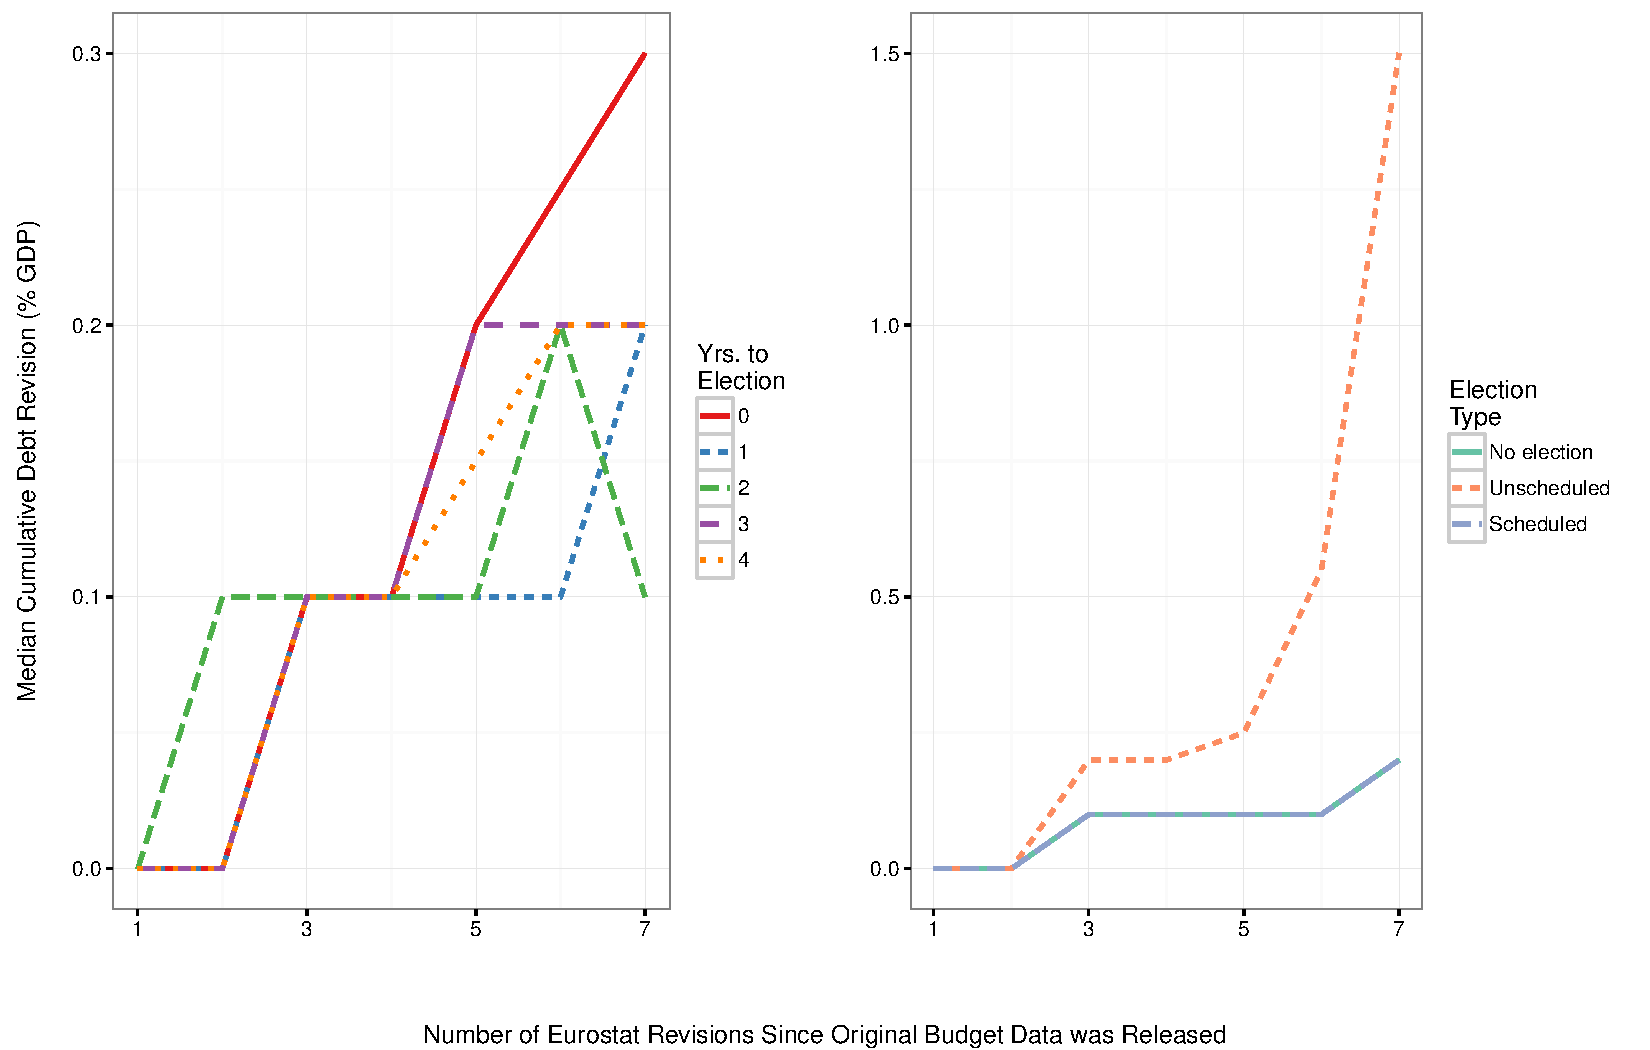
\includegraphics[scale=0.55]{figures/median_debt_revisions.pdf}
    \end{center}
\end{figure}

This measure of rule stretching is related to the dependent variable that is most common in work on `creative accounting', namely the so-called `stock-flow adjustment' (e.g., \citealt{vonHagenWolff2006}, \citealt{Alt2014}; see also \citealt{Seiferling2013} on the technical details).  This term refers to the accounting difference between a country's change in its debt burden and its budget deficit, where positive numbers indicate that debts grew more than deficits.  \cite{vonHagenWolff2006} find that there are more such adjustments when the deficit fiscal rule of 3 percent is in force in Europe, or after 1997.  Our dependent variable here represents an outside agency's evaluation of whether the figures a given member state reports are correct.  One issue on stock-flow adjustments that make them more problematic for our paper is how European accounting rules consider equity injections into public companies as well as transactions in financial assets. Both affect debts but do not affect deficits. Stock-flow adjustments, therefore, would change significantly when governments intervene in the financial sector--purchases of equity in banks as part of recapitalization or the nationalization of banks.  An advantage of our measure is that we can check whether there was rule stretching even during times of high financial stress when governments took action.

Before moving onto the regression analysis let's examine descriptive statistics of our cumulative debt revisions under different conditions related to our non-interactive hypotheses. Figure \ref{median_debt_revisions} shows the median cumulative Eurostat debt revisions in our sample under such conditions.\footnote{Below we discuss these variables in detail. In figures \ref{median_debt_revisions} and \ref{median_deficit_revisions} in the Online Appendix we use the original electoral timing variable, not the reversed scale as, in this representation, the original scale is easier to interpret.} The upper left-panel indicates that revisions are higher for budget data released in years with elections. Cumulative revisions are similar regardless of election timing until the fifth revision. Over the next two revisions, the median cumulative revision for non-election years remains between 0.1 and 0.2 percent of GDP. In contrast, median debt revisions for election years increase to 0.3 percent of GDP by the seventh revision. In the upper right-panel of Figure \ref{median_debt_revisions} we see that the median revision for debt data released in years with unscheduled elections is much higher by the seventh revision (about 1.5 percent of GDP) than for years with scheduled elections or no elections (both are about 0.2 percent of GDP). Again, the divergence in the magnitude of the data revisions largely begins from the fifth time that Eurostat examines the numbers. These descriptive findings are indicative of politicians engaging in fiscal rule stretching in election years, especially if they have impromptu elections.

The lower two panels of Figure \ref{median_debt_revisions} show median debt revisions for countries in and out of an Excessive Deficit Procedure and euro membership. The ultimate median debt revision of 0.25 percent of GDP for countries in EDP enforcement is more than double that for countries without EDP enforcement (lower left-panel). Euro members have a higher median debt data revision than non-eurozone members (upper right-panel). Both of these findings suggest that the external audience may also be an important motivator for fiscal rule stretching.

\subsection{Right-hand variables}

We use Gandrud's \citeyearpar{gandrudYrcurnt} \emph{years to election} variable in the following regressions. The variable counts down from the year that is the furthest away from the next scheduled election. Election years are recorded as zero, regardless of whether they were scheduled or not. To make the marginal effect estimates from the following regressions more intuitive--i.e. so that a positive coefficient indicates that being closer to an election is associated with an increase in debt data revisions, we reversed the direction of the election timing scale.\footnote{I.e. for each observed election timing value $x$ for country $i$ and year $t$: $\mathrm{Max}(\mathrm{X}) - x_{i,t}$.}

Not only do we expect that governments are more likely to use rule stretching as elections approach, but that rule stretching should be more prevalent when governments are not able to choose when the election occurs so as to present themselves in the best fiscal light to voters, as well as international institutions and investors that they need to maintain policies that are popular with voters. As such, we also include a categorical variable indicating \emph{election type}. It codes country-years as having a scheduled election, unscheduled election, or no election. The variable is based on \cite{Brender2008}, which was updated and corrected by \cite{hallerbergWehner2015} through 2010. We updated it through 2013.\footnote{We used information from the NSD European Elections Database available at \url{http://www.nsd.uib.no/european_election_database}. Accessed February 2016.} Based on our theoretical framework and what we saw in the descriptive statistics, we expect that the revisions will be greater for years when there is an unscheduled election. See the Online Appendix for the list of country-years in our sample with unscheduled elections.

To examine how responding to financial market stress may exacerbate governments' fiscal accounting rule stretching behavior, we included Duprey et al.'s \citeyearpar{ThibautDuprey2015} measure of financial market stress. Political economy research has tended to rely on dichotomous financial crisis measures from \cite{Laeven2012} and \cite{ReinhartRog2010} that are hand-coded \emph{post hoc}. Problems with these measures are well known \citep[see][]{finstress_paper}. Duprey et al.'s measure has the advantage of being continuous, monthly, and based on a clearly reproducible methodology. They found their indicator for 27 EU member states by measuring co-movements in key financial market characteristics such as equity, bond market, and foreign exchange volatility. This financial market stress variable is able to vary between zero and one, with higher values indicating more financial market stress. To make this monthly measure comparable with our other variables, we found yearly averages. In the sample the variable falls between 0.02 and 0.57.

We hypothesize that the effect of election timing on rule stretching will increase at higher levels of financial market stress. So in the following discussion we focus on interactions between financial market stress and the election timing and election type variables.

One way we examined the role of external audiences on revisions was with a binary variable that was one when a country was in an \emph{excessive deficit procedure} and zero otherwise. The majority of this data was from \cite{baergHallerberg2016}, which we updated from 2003 through 2004 and from 2013 through 2015.\footnote{We used information from the European Commission available at: \url{http://ec.europa.eu/economy_finance/economic_governance/sgp/corrective_arm/index_en.htm}. Accessed February 2016.}  Being in an Excessive Deficit Procedure could have both a positive and/or negative effect on revisions. On the one hand we may expect countries in EDPs to engage in more rule stretching in order to lower their debts and get out. Conversely, an important consideration in how to enforce the EDP is a government's good faith in returning to compliance. Fiscal rule stretching may be viewed as a bad faith move. As such countries subject to SGP enforcement may be less likely to rule stretch. Given these competing pressures, perhaps governments in EDP rule stretch more when the short-term benefits outweigh the longer-term costs of being discovered. A clear short-term benefit would be reducing the need to cut back spending in years when maintaining government spending is most important, e.g. close to elections. As such, we interacted being in an EDP with election timing.

All member states are covered under the Stability and Growth Pact and so could be put in an EDP. However, non-eurozone members, such as the United Kingdom, face weaker or non-existent enforcement actions if they breach the SGP's limits. As such, we might expect that higher revisions would be associated with being outside of the \emph{eurozone}. Conversely, inspired by \cite{clark2003}, perhaps countries in the eurozone--having fixed exchange rates--need to rely more on rule stretching and so eurozone membership is positively associated with revisions. Because of these conflicting predictions, we do not have strong priors on the unconditional effect of eurozone membership.

However, there is a clear interactive possibility that we consider. Perhaps countries that have higher debts and so are in threat of, or have actually breached, the SGP's limits will be more likely to rule stretch. We would expect that countries in the eurozone specifically would be more likely to rule stretch when their debts are close to and above 60 percent of GDP. Rule stretching in this situation may help them, at least temporarily, stay or get under the SGP's 60 percent debt to GDP limit. A such, we gathered data on \emph{gross central government debt} as a percentage of GDP reported by the World Bank's Development Indicators.\footnote{Available at: \url{http://data.worldbank.org/data-catalog/world-development-indicators}. Accessed December 2015.} We then interacted this variable with \emph{eurozone membership} to see if being in the eurozone specifically gave governments added pressure to stay under the SGP's 60 percent limit.\footnote{The SGP also specifies a 3 percent of GDP deficit. This limit was in many ways the focus of EDP enforcement much more so than the 60 percent of GDP debt limit until the advent of the eurozone debt crisis. To examine the role that deficit levels may play on debt revisions, we gathered data on \emph{general government deficits} as a percentage of GDP from Eurostat. The data is available at: \url{http://ec.europa.eu/Eurostat/} (accessed December 2015.) We used this data in regressions where deficit revisions are modeled. See the Appendix for results.} Note that the debt level data is revised data. Therefore, we expect the effect of this variable on revisions to occur at higher observed levels on the revised data. Governments should rule stretch more for years with debts somewhat above 60 percent of GDP in data that is ultimately revised debt data.

To measure \emph{fiscal transparency}, we use a fiscal transparency index created by \cite{Wang2015}. They measure the degree to which and what type of fiscal data is reported to the International Monetary Fund from 2003 to 2013. Their index ranged from zero to 100 (the maximum possible extent) in our sample of EU member states. We also examined if economic growth as measured by year-over-year GDP growth (percentage) would affect revisions.\footnote{From the World Bank Development Indicators. Indicator ID NY.GDP.MKTP.KD.ZG. Accessed February 2016.} Perhaps governments facing broad economic shocks have incentives to rule stretch more \citep{DeCastro2013}. We used the budget \emph{contracts} institutions (as opposed to institutions that delegate budget responsibility to a ministry of finance) variable from \cite{hallerberg2007design} and \cite{hallerbergstrauch2009}. We may expect that more contractual budgetary institutions have more accurate budget numbers the first time around. The variable ranges from 0.19 to 1 in our sample with higher values indicating more contractual institutions. \todo{Mark: can you look at the previous paragraph to see if the citations are correct and it makes sense}

\section{Empirical tests: results}

Table \ref{debt_results} shows results from linear regressions with cumulative debt revisions as the dependent variable. Because cumulative debt revisions are autoregressive, we also include one-period lagged cumulative debt revisions on the right-hand side in all models. All models also include country fixed effects to account for unobserved country variation. The direction of the country effects is as expected. For example, Greece was more likely to have upward revisions and Luxembourg was more likely to have downward debt revisions (results not shown). Because a number of the variables are logically highly correlated with each other (e.g., countries under an EDP have high debts), we ran our models in a step-wise fashion.

Central government debt was (weakly at the 10\% level) associated with debt revisions in many non-interactive models. The direction of the effect is as expected: countries with higher debt levels were more likely to have debt data that Eurostat revised upwards. Governments with high debts appear to be more likely to engage in fiscal rule stretching. This could be because they have increased incentives--from voters, the EU, and sovereign bond investors--to decrease or at least slow the increase in their debts.

We expect that eurozone members with debt levels at around or above the 60 percent SGP limit would be more likely to engage in fiscal rule stretching. The upper left-panel of Figure \ref{me_comb} shows the marginal effect of eurozone membership at various debt levels. We can see that the effect is positive--eurozone members with higher debt levels are more likely to have revised debt numbers. Interestingly, this effect becomes statistically significant at the 5 percent level when debt is above the 60 percent of GDP SGP limit in the revised data. Note that the original debt to GDP figures were often lower; closer to the 60 percent limit.

Using an interaction between euro membership and election timing (not shown) we examined if the electoral timing effect is particular to countries in the eurozone who cannot use monetary policy to boost the economy before elections. The interaction was not statistically significant at any standard level. So, the evidence points to the electoral timing effect being general to European countries regardless of eurozone membership. This may likely be partially the result of the fact that while countries such as the United Kingdom have monetary policy control, this control is wielded by an independent central bank. As such, governments in all of these countries are largely unable to use monetary policy to boost their re-election chances and so turn to techniques such as fiscal rule stretching to improve their image with voters.

We did not find evidence that once countries are in an Excessive Deficit Procedure that they are unconditionally more likely to present debt figures that Eurostat revises upwards. This is possibly because of the ambiguous benefit of rule stretching when under the EDP. Countries might be able to get their debts under the SGP limit with such optimistic accounting, but once revealed, these actions could be seen as bad faith efforts leading to further penalties. Also, we did not find evidence for an interaction between being in an EDP and eurozone membership (not shown), suggesting that counter to our hypothesis countries in the eurozone facing an EDP are not more likely to rule stretch. There is, however, evidence that debt revisions are higher for particularly important years: those close to elections. This evidence can be seen in the upper right-panel of Figure \ref{me_comb} which shows the marginal effect of being in an EDP at various distances from an election. Being in an EDP puts constraints on a government's budget, which they may want to have eased in order to provide spending that pleases voters. This finding demonstrates how international and domestic electoral incentives can interact to heighten rule stretching.

There is evidence that having an unscheduled election has the hypothesized non-interactive effect on debt revisions. We estimate that having an unscheduled election is associated with larger cumulative Eurostat debt data revisions later on. We found some evidence (at the 10 percent significance level) for an unconditional electoral timing effect, where the closer to an election a government is, the more debt revisions that there are.

How does financial market stress impact the electoral effects? We hypothesised that they should be stronger at higher levels of stress. In the lower left-panel of Figure \ref{me_comb} we can see that the marginal effect of moving a year closer to an election at increasing levels of financial market stress increases debt revisions. From this plot, we estimate that at low levels of stress, there is no statistically significant effect of moving a year closer to an election on cumulative debt revisions. However, at higher levels of stress, e.g. above 0.4 (for context, the United Kingdom and Greece during the heights of their crises had financial market stress scores somewhat above 0.4), moving a year closer to an election is associated with a 0.2 percent of GDP upward revision by Eurostat to the government's debt data. In the lower right-panel of Figure \ref{me_comb} we see a similar directional effect for having an unscheduled election--rather than a scheduled election or no election. At high levels of financial market stress having an unscheduled election has a large--about 1.5 to 2 percentage points of GDP--estimated impact on revisions.\footnote{Perhaps governments that face higher levels of financial market stress are more likely to call unscheduled elections. In the Online Appendix we investigate this possible endogeneity. We do not find evidence that unscheduled elections are more likely at higher levels of financial market stress.}

Fiscal transparency was positively associated with debt revisions in our data set. This suggests that governments with more open budgets may rely more on esoteric ways of improving the short-term appearance of their fiscal policies in the absence of the ability to hide these creative accounting. At the same time, it may be easier for Eurostat to catch rule stretching in more transparent countries. From an office-seeking incumbent politician's short-term perspective, this is not much of a deterrent as it may take Eurostat two to three years to make these corrections.

The estimated coefficient for GDP growth was not statistically significant at conventional levels\footnote{An interaction between GDP growth and election type was significant at the 10 percent level. However, this could be largely because GDP declines are associated with financial market stress. Estimates from a financial market stress interaction was stronger and this model's adjusted $R^{2}$ was higher.} We found no evidence that budget contract institutions by impacted debt revisions. Because Greece is a considerable outlier in terms of its debt revisions, we also ran our models with Greece omitted from the sample. The results of these models are shown in the Online Appendix. Removing Greece did not change the substantive significance of the findings, suggesting that the fiscal rule stretching behaviour we have identified is not confined to Greece, but is instead a wider phenomenon in Europe.


\begin{figure}
    \caption{Marginal Effects of Various External and Domestic Audience Conditions on \textbf{Debt} Revisions}
    \label{me_comb}

    \begin{center}
        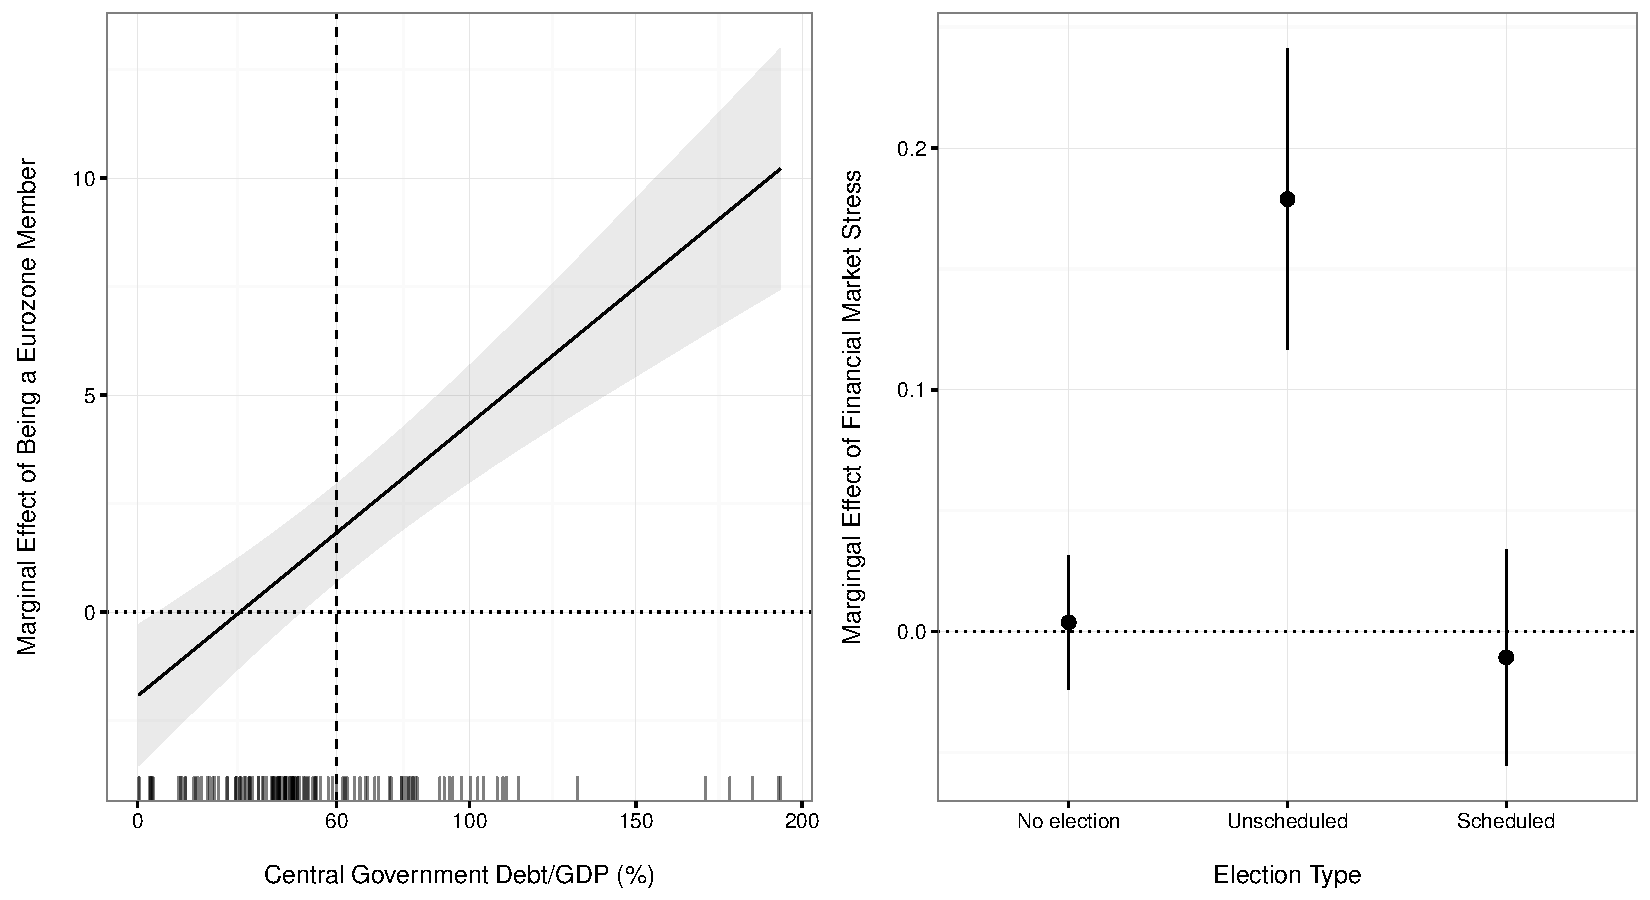
\includegraphics[scale=0.55]{figures/debt_me_comb.pdf}
    \end{center}

	{\scriptsize{Shaded areas represent 95\% confidence intervals.\\
    The dashed vertical line in the upper left-panel indicates a debt level of 60\% of GDP. This is the Stability and Growth Pact debt limit past which member states can be put into an Excessive Deficit Procedure.}}

\end{figure}

\begin{landscape}
    
% Table created by stargazer v.5.2 by Marek Hlavac, Harvard University. E-mail: hlavac at fas.harvard.edu
% Date and time: Fri, Feb 12, 2016 - 14:39:59
\begin{table}[!htbp] \centering 
  \caption{Linear Regression Estimation of \textbf{Debt} Revisions} 
  \label{debt_results} 
\tiny 
\begin{tabular}{@{\extracolsep{5pt}}lccccccccccc} 
\\[-1.8ex]\hline 
\hline \\[-1.8ex] 
 & \multicolumn{11}{c}{\textit{Dependent variable:}} \\ 
\cline{2-12} 
\\[-1.8ex] & \multicolumn{11}{c}{Cumulative Debt Revisions} \\ 
\\[-1.8ex] & (1) & (2) & (3) & (4) & (5) & (6) & (7) & (8) & (9) & (10) & (11)\\ 
\hline \\[-1.8ex] 
 Cum. Revisions (lag) & 0.628$^{***}$ & 0.757$^{***}$ & 0.626$^{***}$ & 0.731$^{***}$ & 0.554$^{***}$ & 0.536$^{***}$ & 0.641$^{***}$ & 0.640$^{***}$ & 0.634$^{***}$ & 0.681$^{***}$ & 0.634$^{***}$ \\ 
  & (0.021) & (0.021) & (0.021) & (0.022) & (0.026) & (0.026) & (0.021) & (0.021) & (0.022) & (0.025) & (0.022) \\ 
  & & & & & & & & & & & \\ 
 Election Timing & 0.047$^{*}$ &  & $-$0.031 &  &  &  &  &  & $-$0.064 &  & $-$0.028 \\ 
  & (0.027) &  & (0.047) &  &  &  &  &  & (0.049) &  & (0.040) \\ 
  & & & & & & & & & & & \\ 
 Unscheduled Elect. &  & 0.229$^{*}$ &  & $-$0.560$^{**}$ &  &  &  &  &  & $-$0.576$^{**}$ &  \\ 
  &  & (0.132) &  & (0.235) &  &  &  &  &  & (0.248) &  \\ 
  & & & & & & & & & & & \\ 
 Scheduled Elect. &  & $-$0.001 &  & $-$0.057 &  &  &  &  &  & $-$0.157 &  \\ 
  &  & (0.073) &  & (0.128) &  &  &  &  &  & (0.150) &  \\ 
  & & & & & & & & & & & \\ 
 Financial Stress & 0.039 & 0.191 & $-$1.082$^{*}$ & $-$0.049 &  &  &  &  & $-$1.380$^{**}$ & $-$0.001 & 0.075 \\ 
  & (0.327) & (0.257) & (0.643) & (0.278) &  &  &  &  & (0.651) & (0.331) & (0.343) \\ 
  & & & & & & & & & & & \\ 
 Gen. Gov. Deficit &  &  &  &  & $-$0.004 & 0.010 &  &  &  &  &  \\ 
  &  &  &  &  & (0.011) & (0.011) &  &  &  &  &  \\ 
  & & & & & & & & & & & \\ 
 Cent. Gov. Debt &  &  &  &  & 0.004$^{*}$ & 0.004$^{*}$ &  &  &  &  &  \\ 
  &  &  &  &  & (0.002) & (0.002) &  &  &  &  &  \\ 
  & & & & & & & & & & & \\ 
 Euro Member &  &  &  &  & 0.233 & $-$0.479$^{*}$ & $-$0.006 & $-$0.066 &  &  &  \\ 
  &  &  &  &  & (0.183) & (0.272) & (0.194) & (0.201) &  &  &  \\ 
  & & & & & & & & & & & \\ 
 EDP &  &  &  &  &  &  & 0.163$^{**}$ & 0.041 & 0.175$^{**}$ & 0.083 & $-$0.145 \\ 
  &  &  &  &  &  &  & (0.080) & (0.131) & (0.082) & (0.081) & (0.155) \\ 
  & & & & & & & & & & & \\ 
 Elect. Timing*Fin. Stress &  &  & 0.506$^{**}$ &  &  &  &  &  & 0.658$^{***}$ &  &  \\ 
  &  &  & (0.250) &  &  &  &  &  & (0.252) &  &  \\ 
  & & & & & & & & & & & \\ 
 Unscheduled.Elect*Fin. Stress &  &  &  & 5.818$^{***}$ &  &  &  &  &  & 6.493$^{***}$ &  \\ 
  &  &  &  & (1.443) &  &  &  &  &  & (1.524) &  \\ 
  & & & & & & & & & & & \\ 
 Scheduled.Elect*Fin. Stress &  &  &  & 0.384 &  &  &  &  &  & 0.980 &  \\ 
  &  &  &  & (0.731) &  &  &  &  &  & (0.815) &  \\ 
  & & & & & & & & & & & \\ 
 Cent. Gov. Debt*Euro &  &  &  &  &  & 0.011$^{***}$ &  &  &  &  &  \\ 
  &  &  &  &  &  & (0.003) &  &  &  &  &  \\ 
  & & & & & & & & & & & \\ 
 EDP*Euro &  &  &  &  &  &  &  & 0.191 &  &  &  \\ 
  &  &  &  &  &  &  &  & (0.162) &  &  &  \\ 
  & & & & & & & & & & & \\ 
 Elect. Timing*EDP &  &  &  &  &  &  &  &  &  &  & 0.137$^{**}$ \\ 
  &  &  &  &  &  &  &  &  &  &  & (0.057) \\ 
  & & & & & & & & & & & \\ 
 Constant & 0.648$^{***}$ & 0.361$^{**}$ & 0.831$^{***}$ & 0.353$^{**}$ & 0.251 & 0.316 & 0.658$^{**}$ & 0.688$^{***}$ & 0.807$^{***}$ & 0.343$^{**}$ & 0.752$^{***}$ \\ 
  & (0.188) & (0.151) & (0.208) & (0.152) & (0.309) & (0.308) & (0.255) & (0.257) & (0.209) & (0.160) & (0.203) \\ 
  & & & & & & & & & & & \\ 
\hline \\[-1.8ex] 
Country FE? & Yes & Yes & Yes & Yes & Yes & Yes & Yes & Yes & Yes &  &  \\ 
Observations & 1,494 & 1,189 & 1,494 & 1,189 & 1,230 & 1,230 & 1,371 & 1,371 & 1,345 & 1,047 & 1,345 \\ 
R$^{2}$ & 0.546 & 0.655 & 0.547 & 0.660 & 0.397 & 0.403 & 0.546 & 0.546 & 0.548 & 0.636 & 0.548 \\ 
Adjusted R$^{2}$ & 0.537 & 0.646 & 0.538 & 0.651 & 0.384 & 0.390 & 0.536 & 0.536 & 0.538 & 0.625 & 0.537 \\ 
\hline 
\hline \\[-1.8ex] 
\textit{Note:}  & \multicolumn{11}{r}{$^{*}$p$<$0.1; $^{**}$p$<$0.05; $^{***}$p$<$0.01} \\ 
\end{tabular} 
\end{table} 

\end{landscape}


\section{Conclusion}

We have sought to understand government debt rule stretching behavior in Europe, especially during periods of financial market stress and crises. The European Union provides a unique opportunity for studying this behavior as it has a common set of statistical rules--the ESA--and has a highly independent monitor--Eurostat--that regularly revisits and revises member state balance sheet statistics to ensure that they are in line with these rules.

We significantly deepen findings in previous work that elections are associated with revisions to government finance figures. We specifically examine behavior during unscheduled elections and periods of financial market stress. We find that government debt rule stretching for domestic audiences is much more prevalent during financial crises and when elections are unscheduled, when governments have few opportunities to affect economic fundamentals in time for voters to appreciate it.

We also explore how the European-level audience affects rule stretching behaviour. We found that policy-makers in the eurozone--who are subject to stronger Excessive Deficit Procedure enforcement--are cognizant of the Stability and Growth Pact's 60 percent debt limit and possibly use rule stretching in attempts to be below it. Domestic and European-level incentives to rule stretch appear to interact with each other as countries in Excessive Deficit Procedure enforcement are more likely to rule stretch on their debt data when they are closer to elections.

A major takeaway from our work is that even among a group of developed economies with generally strong economic institutions, fiscal rule stretching is common and can significantly affect our knowledge about government spending and financial obligations. This is especially true during financial market stress. European-level debt limits and the enforcement of these limits also appears to encourage rule stretching in certain circumstances. As such independent government accounting agencies, such as Eurostat, are a crucial component of `getting the numbers right', even if it takes a few years.


\clearpage

\bibliographystyle{apsr}
\bibliography{main.bib}

\pagebreak
\renewcommand{\thepage}{A-\arabic{page}}\setcounter{page}{1}
\renewcommand{\thesection}{Appendix \arabic{section}}\setcounter{section}{0}
\renewcommand{\thetable}{A-\arabic{table}}\setcounter{table}{0}
\renewcommand{\thefigure}{A-\arabic{figure}}\setcounter{figure}{0}
\clearpage

\section*{Online Appendix}

\subsection*{Independent National Debt Rule Monitors}

All EU countries have an independent supranational debt rule monitor--Eurostat. Six member states had additional national independent debt rule monitors during our sampling period. Table \ref{indep_monitors} shows the list of countries in our sample with such national institutions. This data is from \cite{bova2015rules}.\footnote{Data available at: \url{http://www.imf.org/external/datamapper/FiscalRules/map/map.htm}. Accessed February 2016.}

% latex table generated in R 3.2.3 by xtable 1.8-2 package
% Wed Feb 24 09:15:08 2016
\begin{table}[ht]
\centering
\caption{Start and End Years (if any) of Independent National Debt Rule Monitors, from \cite{bova2015rules}} 

\label{indep_monitors}
\begin{tabular}{lrr}
  \hline
Country & Start & End \\ 
  \hline
Lithuania & 2004 &  \\ 
  Netherlands & 2003 &  \\ 
  Poland & 2004 & 2012 \\ 
  Romania & 2013 &  \\ 
  Slovakia & 2012 &  \\ 
  United Kingdom & 2010 &  \\ 
   \hline
\end{tabular}
\end{table}


\subsection*{Crisis and the possibility of selection into unscheduled elections}

We examined whether or not governments select into unscheduled elections according to the prevailing level of financial market stress. Table \ref{unschedule_list} shows the list of country-years with unscheduled elections in our sample. Table \ref{finstress_endog} shows results from a logistic regression where we tried to predict having an unscheduled election in a year for our sample based on annual average stress level. We can see that there is a null result. We made a similar finding when running a similar model with lagged financial market stress and a  multinomial logistic regression (both not shown), with unscheduled and scheduled elections as categories and no election as the reference category.

% latex table generated in R 3.2.3 by xtable 1.8-2 package
% Wed Mar  2 12:41:48 2016
\begin{table}[ht]
\centering
\caption{Country-years With Unscheduled Elections in Our Sample} 
\label{unschedule_list}
\begin{tabular}{lr}
  \hline
Country & Unscheduled Election Year \\ 
  \hline
Austria & 2008 \\ 
  Belgium & 2010 \\ 
  Denmark & 2007 \\ 
  Germany & 2005 \\ 
  Greece & 2007 \\ 
  Greece & 2009 \\ 
  Greece & 2012 \\ 
  Ireland & 2011 \\ 
  Italy & 2008 \\ 
  Latvia & 2011 \\ 
  Netherlands & 2003 \\ 
  Netherlands & 2012 \\ 
  Poland & 2007 \\ 
  Portugal & 2005 \\ 
  Portugal & 2011 \\ 
  Slovakia & 2012 \\ 
  Slovenia & 2011 \\ 
  Spain & 2011 \\ 
  United Kingdom & 2005 \\ 
   \hline
\end{tabular}
\end{table}



% Table created by stargazer v.5.2 by Marek Hlavac, Harvard University. E-mail: hlavac at fas.harvard.edu
% Date and time: Fri, May 06, 2016 - 09:17:46
\begin{table}[!htbp] \centering 
  \caption{Logistic Regression Estimation of Having an Unscheduled Election} 
  \label{finstress_endog} 
\begin{tabular}{@{\extracolsep{5pt}}lc} 
\\[-1.8ex]\hline 
\hline \\[-1.8ex] 
 & \multicolumn{1}{c}{\textit{Dependent variable:}} \\ 
\cline{2-2} 
\\[-1.8ex] & Unscheduled Election \\ 
\hline \\[-1.8ex] 
 Financial Stress & 2.246 \\ 
  & (2.435) \\ 
  & \\ 
 Constant & $-$2.612$^{**}$ \\ 
  & (1.107) \\ 
  & \\ 
\hline \\[-1.8ex] 
Country FE? & Yes \\ 
Observations & 281 \\ 
Log Likelihood & $-$56.469 \\ 
Akaike Inf. Crit. & 168.939 \\ 
\hline 
\hline \\[-1.8ex] 
\textit{Note:}  & \multicolumn{1}{r}{$^{*}$p$<$0.1; $^{**}$p$<$0.05; $^{***}$p$<$0.01} \\ 
\end{tabular} 
\end{table} 


\subsection*{Omitting Greece}

Greece has very large debt revisions in our sample. For each year from 2007 through 2011 Greece's debt statistics were cumulatively revised upward by over 10 percentage points. To examine if this one country was driving our election results, we reran our models omitting Greece. The results of this exercise are shown in Table \ref{results_no_greece}. We can see that the substantive findings from reported from models in the full sample in Table \ref{debt_results} are largely unchanged in models excluding Greece.

\begin{landscape}
    
% Table created by stargazer v.5.2 by Marek Hlavac, Harvard University. E-mail: hlavac at fas.harvard.edu
% Date and time: Thu, Oct 27, 2016 - 13:37:05
\begin{table}[!htbp] \centering 
  \caption{Linear Regression Estimation of Debt Revisions (Excluding Greece)} 
  \label{results_no_greece} 
\tiny 
\begin{tabular}{@{\extracolsep{5pt}}lcccccccccc} 
\\[-1.8ex]\hline 
\hline \\[-1.8ex] 
 & \multicolumn{10}{c}{\textit{Dependent variable:}} \\ 
\cline{2-11} 
\\[-1.8ex] & \multicolumn{10}{c}{Cumulative Debt Revisions} \\ 
\\[-1.8ex] & (1) & (2) & (3) & (4) & (5) & (6) & (7) & (8) & (9) & (10)\\ 
\hline \\[-1.8ex] 
 Revised Cent. Gov. Debt & 0.023$^{*}$ & 0.016$^{*}$ & 0.016 & 0.016 & 0.015 & 0.009 & 0.028$^{**}$ & 0.017 & 0.056$^{***}$ & 0.029$^{**}$ \\ 
  & (0.010) & (0.008) & (0.011) & (0.011) & (0.011) & (0.010) & (0.009) & (0.011) & (0.012) & (0.010) \\ 
  & & & & & & & & & & \\ 
 Euro Member & 1.825$^{*}$ & $-$1.971 & 1.408 & 1.522 & 1.426 & 1.259 & 2.142$^{*}$ & 1.543 & 0.011 & $-$1.450 \\ 
  & (0.853) & (0.998) & (0.911) & (0.911) & (0.920) & (0.834) & (0.830) & (0.904) & (0.871) & (0.982) \\ 
  & & & & & & & & & & \\ 
 EDP & 0.158 &  &  &  &  &  &  &  &  & $-$0.142 \\ 
  & (0.389) &  &  &  &  &  &  &  &  & (0.355) \\ 
  & & & & & & & & & & \\ 
 Election Timing &  &  & 0.178 & $-$0.429 &  &  &  & $-$0.416 &  &  \\ 
  &  &  & (0.108) & (0.461) &  &  &  & (0.456) &  &  \\ 
  & & & & & & & & & & \\ 
 Unscheduled Elect. &  &  &  &  & 1.217$^{*}$ & $-$7.741$^{***}$ &  &  &  & $-$5.342$^{**}$ \\ 
  &  &  &  &  & (0.591) & (1.996) &  &  &  & (1.867) \\ 
  & & & & & & & & & & \\ 
 Scheduled Elect. &  &  &  &  & $-$0.007 & 0.618 &  &  &  & 0.733 \\ 
  &  &  &  &  & (0.368) & (1.332) &  &  &  & (1.245) \\ 
  & & & & & & & & & & \\ 
 Financial Stress &  &  & 0.016 & $-$0.016 & 0.014 & 0.004 &  & 0.00002 &  & $-$0.041 \\ 
  &  &  & (0.017) & (0.029) & (0.017) & (0.017) &  & (0.030) &  & (0.022) \\ 
  & & & & & & & & & & \\ 
 Fiscal Transparency &  &  &  &  &  &  & 0.008 & 0.004 &  &  \\ 
  &  &  &  &  &  &  & (0.010) & (0.010) &  &  \\ 
  & & & & & & & & & & \\ 
 GDP Growth &  &  &  &  &  &  & 0.072 & 0.107$^{*}$ &  & 0.053 \\ 
  &  &  &  &  &  &  & (0.046) & (0.050) &  & (0.043) \\ 
  & & & & & & & & & & \\ 
 Contracts &  &  &  &  &  &  &  &  & 3.369 &  \\ 
  &  &  &  &  &  &  &  &  & (4.960) &  \\ 
  & & & & & & & & & & \\ 
 Debt * Euro &  & 0.064$^{***}$ &  &  &  &  &  &  &  & 0.075$^{***}$ \\ 
  &  & (0.012) &  &  &  &  &  &  &  & (0.016) \\ 
  & & & & & & & & & & \\ 
 Elect. Timing * Fin. Stress &  &  &  & 0.012 &  &  &  & 0.012 &  &  \\ 
  &  &  &  & (0.009) &  &  &  & (0.009) &  &  \\ 
  & & & & & & & & & & \\ 
 Unscheduled Elect. * Fin. Stress &  &  &  &  &  & 0.175$^{***}$ &  &  &  & 0.110$^{**}$ \\ 
  &  &  &  &  &  & (0.038) &  &  &  & (0.036) \\ 
  & & & & & & & & & & \\ 
 Scheduled Elect. * Fin. Stress &  &  &  &  &  & $-$0.014 &  &  &  & $-$0.014 \\ 
  &  &  &  &  &  & (0.028) &  &  &  & (0.027) \\ 
  & & & & & & & & & & \\ 
 Constant & 8.294$^{***}$ & 7.750$^{***}$ & 8.192$^{***}$ & 9.857$^{***}$ & 8.609$^{***}$ & 9.923$^{***}$ & 7.185$^{***}$ & 8.259$^{***}$ & 4.614 & 8.003$^{***}$ \\ 
  & (1.687) & (1.450) & (1.638) & (2.042) & (1.641) & (1.560) & (1.778) & (2.143) & (4.663) & (1.584) \\ 
  & & & & & & & & & & \\ 
\hline \\[-1.8ex] 
Country FE? & Yes & Yes & Yes & Yes & Yes & Yes & Yes & Yes & Yes & Yes \\ 
Observations & 118 & 123 & 123 & 123 & 123 & 123 & 123 & 123 & 112 & 118 \\ 
R$^{2}$ & 0.695 & 0.760 & 0.698 & 0.703 & 0.703 & 0.762 & 0.697 & 0.718 & 0.746 & 0.820 \\ 
Adjusted R$^{2}$ & 0.604 & 0.692 & 0.608 & 0.611 & 0.610 & 0.681 & 0.607 & 0.623 & 0.672 & 0.746 \\ 
\hline 
\hline \\[-1.8ex] 
\textit{Note:}  & \multicolumn{10}{r}{$^{*}$p$<$0.05; $^{**}$p$<$0.01; $^{***}$p$<$0.001} \\ 
\end{tabular} 
\end{table} 

\end{landscape}

\subsection*{Deficit Revisions}

In addition to debt revisions explored in the main text, we also explored deficit revisions in a similar manner. First we examine deficit revisions descriptively. Figure \ref{median_deficit_revisions} (similar to Figure \ref{median_debt_revisions} in the main text) shows the cumulative Eurostat deficit revisions in our sample under different electoral conditions. The electoral pattern is somewhat less clear for deficit revisions than debt revisions discussed in the main paper though the effect is in the same theoretical direction as we found in the debt revisions. In the left-panel of Figure \ref{median_deficit_revisions} years far away from a scheduled election--i.e. three and four years from the election--deficits are generally either not revised or slightly revised upwards such that the government ran a slight surplus relative to the original data. Conversely, data for years closer to an election are revised somewhat downward. In other words, governments spent more relative to their income than they had originally reported. The right-panel of Figure \ref{median_deficit_revisions} indicates that both scheduled and unscheduled election years see larger median downward deficit revisions. There appears to be a small cumulative difference between these two types of elections with unscheduled elections having somewhat larger downward revisions by the seventh revision. We see a broadly similar story in left-panel of Figure \ref{median_deficit_revisions_euro_edp} for countries in an EDP as with the debt data. By the end of the revision period, on average downward deficit revisions are higher for countries in an EDP. Interestingly, non-eurozone members had larger deficit revisions than eurozone members. This is the opposite direction of what we found in the debt revisions data.

\begin{figure}
    \begin{center}
        \caption{Median \textbf{Deficit} Revisions for Data Released Under Various Electoral Conditions}
        \label{median_deficit_revisions}
        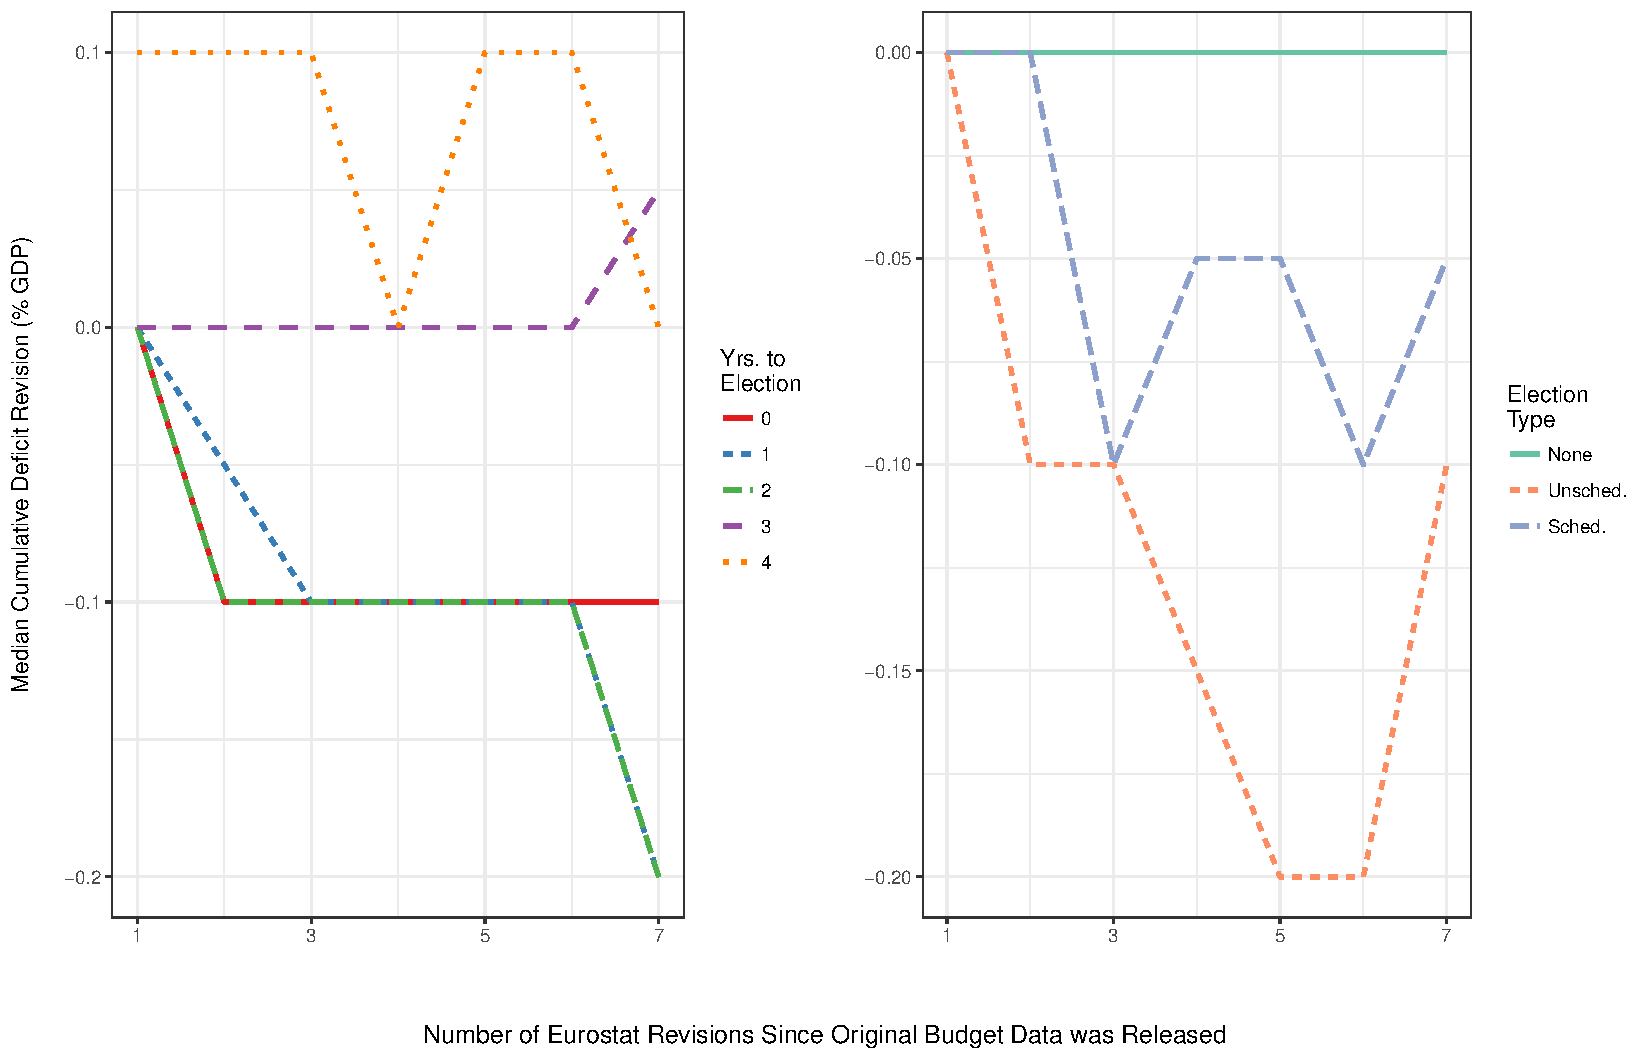
\includegraphics[scale=0.55]{figures/median_deficit_revisions.pdf}
    \end{center}
\end{figure}

\begin{figure}
    \begin{center}
        \caption{Median \textbf{Deficit} Revisions for Data Released Under Various EDP and eurozone conditions}
        \label{median_deficit_revisions_euro_edp}
        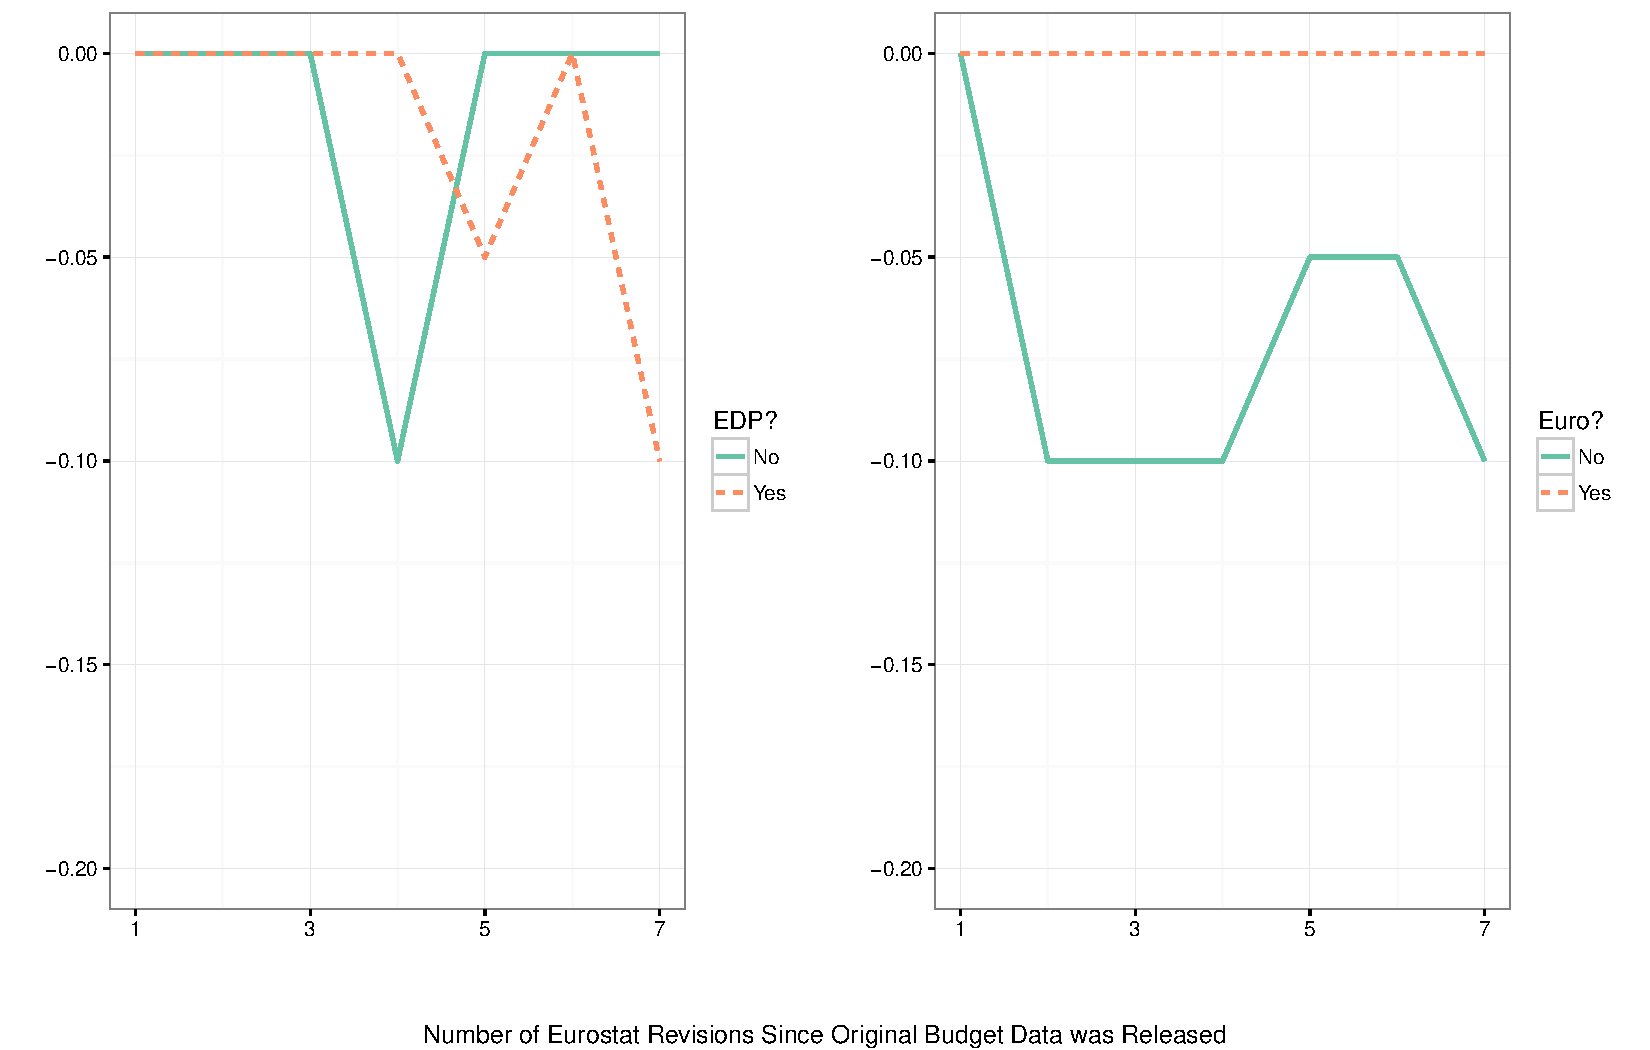
\includegraphics[scale=0.55]{figures/median_deficit_revisions_edp_euro.pdf}
    \end{center}
\end{figure}


We then ran similar models as those found in Table \ref{debt_results} with cumulative deficit revisions as the dependent variable. A difference is that we use deficits rather than debts on the right-hand side. Also, rather than interacting euro membership with debts, in these models we made the more relevant interaction: deficit levels interacted with euro membership. These results are shown in Table \ref{deficit_results}. Having larger deficits is associated with larger deficit revisions, likely as governments use fiscal rule stretching to contain their reported deficits. We largely did not evidence for the electoral effects or their interaction with financial market stress.

\begin{landscape}
    
% Table created by stargazer v.5.2 by Marek Hlavac, Harvard University. E-mail: hlavac at fas.harvard.edu
% Date and time: Thu, Oct 27, 2016 - 13:37:08
\begin{table}[!htbp] \centering 
  \caption{Linear Regression Estimation of Deficit Revisions (Full Sample)} 
  \label{deficit_results} 
\tiny 
\begin{tabular}{@{\extracolsep{5pt}}lcccccccccc} 
\\[-1.8ex]\hline 
\hline \\[-1.8ex] 
 & \multicolumn{10}{c}{\textit{Dependent variable:}} \\ 
\cline{2-11} 
\\[-1.8ex] & \multicolumn{10}{c}{Cumulative Deficit Revisions} \\ 
\\[-1.8ex] & (1) & (2) & (3) & (4) & (5) & (6) & (7) & (8) & (9) & (10)\\ 
\hline \\[-1.8ex] 
 Revised Gen. Gov. Deficit & 0.053$^{***}$ & 0.042$^{*}$ & 0.042$^{*}$ & 0.048$^{***}$ & 0.049$^{***}$ & 0.049$^{***}$ & 0.038$^{**}$ & 0.050$^{***}$ & 0.033$^{**}$ & 0.098$^{**}$ \\ 
  & (0.013) & (0.020) & (0.020) & (0.013) & (0.013) & (0.013) & (0.013) & (0.014) & (0.011) & (0.030) \\ 
  & & & & & & & & & & \\ 
 Euro Member & $-$0.190 & $-$0.180 & $-$0.180 & $-$0.183 & $-$0.192 & $-$0.205 & $-$0.145 & $-$0.179 & $-$0.329 & $-$0.353 \\ 
  & (0.197) & (0.193) & (0.193) & (0.182) & (0.181) & (0.182) & (0.188) & (0.190) & (0.262) & (0.212) \\ 
  & & & & & & & & & & \\ 
 EDP & 0.340$^{**}$ &  &  &  &  &  &  &  &  & 0.346$^{**}$ \\ 
  & (0.104) &  &  &  &  &  &  &  &  & (0.112) \\ 
  & & & & & & & & & & \\ 
 Election Timing &  &  &  & $-$0.014 &  &  &  & $-$0.038 &  &  \\ 
  &  &  &  & (0.027) &  &  &  & (0.124) &  &  \\ 
  & & & & & & & & & & \\ 
 Unscheduled Elect. &  &  &  &  & $-$0.163 & 0.663 &  &  &  & 0.518 \\ 
  &  &  &  &  & (0.153) & (0.640) &  &  &  & (0.661) \\ 
  & & & & & & & & & & \\ 
 Scheduled Elect. &  &  &  &  & 0.115 & $-$0.197 &  &  &  & $-$0.349 \\ 
  &  &  &  &  & (0.090) & (0.369) &  &  &  & (0.427) \\ 
  & & & & & & & & & & \\ 
 Financial Stress &  &  &  & 0.008 & 0.009$^{*}$ & 0.009 &  & 0.007 &  & 0.005 \\ 
  &  &  &  & (0.004) & (0.004) & (0.005) &  & (0.008) &  & (0.006) \\ 
  & & & & & & & & & & \\ 
 Fiscal Transparency &  &  &  &  &  &  & $-$0.001 & $-$0.0003 &  &  \\ 
  &  &  &  &  &  &  & (0.003) & (0.003) &  &  \\ 
  & & & & & & & & & & \\ 
 GDP Growth &  &  &  &  &  &  & $-$0.008 & $-$0.003 &  & $-$0.004 \\ 
  &  &  &  &  &  &  & (0.010) & (0.010) &  & (0.012) \\ 
  & & & & & & & & & & \\ 
 Contracts &  &  &  &  &  &  &  &  & $-$0.669 &  \\ 
  &  &  &  &  &  &  &  &  & (1.999) &  \\ 
  & & & & & & & & & & \\ 
 Debt * Euro &  & $-$0.013 & $-$0.013 &  &  &  &  &  &  & $-$0.042 \\ 
  &  & (0.024) & (0.024) &  &  &  &  &  &  & (0.029) \\ 
  & & & & & & & & & & \\ 
 Elect. Timing * Fin. Stress &  &  &  &  &  & $-$0.017 &  &  &  & $-$0.016 \\ 
  &  &  &  &  &  & (0.013) &  &  &  & (0.013) \\ 
  & & & & & & & & & & \\ 
 Unscheduled Elect. * Fin. Stress &  &  &  &  &  & 0.007 &  &  &  & 0.011 \\ 
  &  &  &  &  &  & (0.008) &  &  &  & (0.009) \\ 
  & & & & & & & & & & \\ 
 Scheduled Elect. * Fin. Stress &  &  &  &  &  &  &  & 0.001 &  &  \\ 
  &  &  &  &  &  &  &  & (0.003) &  &  \\ 
  & & & & & & & & & & \\ 
 Constant & $-$0.322 & $-$0.303 & $-$0.303 & $-$0.654$^{*}$ & $-$0.696$^{*}$ & $-$0.704$^{*}$ & $-$0.265 & $-$0.551 & 0.464 & $-$0.428 \\ 
  & (0.267) & (0.259) & (0.259) & (0.314) & (0.310) & (0.324) & (0.273) & (0.457) & (1.839) & (0.381) \\ 
  & & & & & & & & & & \\ 
\hline \\[-1.8ex] 
Country FE? & Yes & Yes & Yes & Yes & Yes & Yes & Yes & Yes & Yes & Yes \\ 
Observations & 413 & 460 & 460 & 460 & 460 & 460 & 460 & 460 & 423 & 413 \\ 
R$^{2}$ & 0.286 & 0.267 & 0.267 & 0.274 & 0.279 & 0.283 & 0.268 & 0.274 & 0.265 & 0.306 \\ 
Adjusted R$^{2}$ & 0.232 & 0.216 & 0.216 & 0.221 & 0.225 & 0.226 & 0.215 & 0.216 & 0.215 & 0.240 \\ 
\hline 
\hline \\[-1.8ex] 
\textit{Note:}  & \multicolumn{10}{r}{$^{*}$p$<$0.05; $^{**}$p$<$0.01; $^{***}$p$<$0.001} \\ 
\end{tabular} 
\end{table} 

\end{landscape}

\end{document}
